\section{Kunstig intelligens i medisinsk forskning}

\begin{frame}{Kunstig intelligens og hjerneavbildningsdata}
    \begin{tikzpicture}
        \node[] at (-7, -3.25) {};
        \node[] at (7, 3.25) {};

        \inputside{-4.5}{-0.2175}{1.5cm}

        \only<1-2>{
            \node[anchor=west, align=left, font=\normalfont\linespread{0.9}\selectfont] (output) at (3.55, -0.2175) {Klinisk relevant\\prediksjon};
        }

        \only<1>{
            \node[fill=gray!80, minimum width=4cm, minimum height=2.9cm, rounded corners=0.1cm, text=white, draw=black, font=\systemfont, text depth=2.4cm] (rule) at (0, 0) {
                Kunstig nevralt nettverk
            };
            \draw[-stealth] (input) -- ($ (rule.south west) + (0, 1.25) $);
            \draw[-stealth] ($ (rule.south east) + (0, 1.25) $) -- (output);
            \neuron{n00}{($ (rule.south) + (0, 1.25) + (-2*\hsep, -2*\vsep) $)}
            \neuron{n01}{($ (n00) + (0, \vsep) $)}
            \neuron{n02}{($ (n00) + (0, 2*\vsep) $)}
            \neuron{n03}{($ (n00) + (0, 3*\vsep) $)}
            \neuron{n04}{($ (n00) + (0, 4*\vsep) $)}

            \neuron{n10}{($ (n00) + (\hsep, 0.5*\vsep) $)}
            \neuron{n11}{($ (n00) + (\hsep, 1.5*\vsep) $)}
            \neuron{n12}{($ (n00) + (\hsep, 2.5*\vsep) $)}
            \neuron{n13}{($ (n00) + (\hsep, 3.5*\vsep) $)}

            \neuron{n20}{($ (n00) + (2*\hsep, \vsep) $)}
            \neuron{n21}{($ (n00) + (2*\hsep, 2*\vsep) $)}
            \neuron{n22}{($ (n00) + (2*\hsep, 3*\vsep) $)}

            \neuron{n30}{($ (n00) + (3*\hsep, 1.5*\vsep) $)}
            \neuron{n31}{($ (n00) + (3*\hsep, 2.5*\vsep) $)}

            \neuron{n40}{($ (n00) + (4*\hsep, 2*\vsep) $)}

            \foreach \j in {0,...,4} {
                \draw[black, opacity=\edgeopacity] ($ (rule.west) - (0, 0.2175) $) -- (n0\j);
            }

            \foreach \j in {0,...,4} {
                \foreach \k in {0,...,3} {
                    \draw[black, opacity=\edgeopacity] (n0\j) -- (n1\k);
                }
            }
            \foreach \j in {0,...,3} {
                \foreach \k in {0,...,2} {
                    \draw[black, opacity=\edgeopacity] (n1\j) -- (n2\k);
                }
            }
            \foreach \j in {0,...,2} {
                \foreach \k in {0,...,1} {
                    \draw[black, opacity=\edgeopacity] (n2\j) -- (n3\k);
                }
            }
            \draw[black, opacity=\edgeopacity] (n30) -- (n40);
            \draw[black, opacity=\edgeopacity] (n31) -- (n40);
            \draw[black, opacity=\edgeopacity] (n40) -- ($ (rule.south east) + (0, 1.25) $);
        }
        \only<2-3>{
            \cnnarrow{(input.east)}{($ (input.center) + (3, 0) $)}{black}
            \cnn{-2.7}{-0.2175}{0.1}{0.15}{uiogreen}{1}
        }
        \only<2>{
            \cnnarrow{($ (output.west) - (1, 0) $)}{($ (output.west) + (0.1, 0) $)}{black}
        }
        \only<3>{
            \node[anchor=west, align=left, font=\normalfont\linespread{0.9}\selectfont] (output1) at ($ (3.55, -0.2175) + (0, 0.5) $) {Pasient};
            \node[anchor=west, align=left, font=\normalfont\linespread{0.9}\selectfont] (output2) at ($ (3.55, -0.2175) - (0, 0.5) $) {Frisk\\kontroll};
            \cnnarrow{($ (output1.west) - (1, 0.5) $)}{($ (output1.west) + (0.1, 0) $)}{black}
            \cnnarrow{($ (output2.west) - (1, -0.5) $)}{($ (output2.west) + (0.1, 0) $)}{black}
        }
    \end{tikzpicture}
\end{frame}

\newcommand{\pubmed}{
    \begin{tikzpicture}
        \begin{axis}[
            height=5.5cm,
            width=12cm,
            xlabel={År},
            ylabel={Antall publikasjoner},
            axis lines=left,
            xtick pos=bottom,
            ytick pos=left,
            xmin=2000,
            xmax=2025,
            xtick={2000, 2005, 2010, 2015, 2020},
            xticklabels={2000, 2005, 2010, 2015, 2020}
        ]
            \addplot[
                uiogreen,
                thick,
                mark=*
            ] table[col sep=comma, x=Year, y=Count] {data/pubmed.csv};
        \end{axis}
    \end{tikzpicture}
}

\newcommand{\dementia}[1]{
    \begin{tikzpicture}
        \begin{axis}[
            height=5.5cm,
            width=12cm,
            xlabel=År,
            ylabel=Treffsikkerhet,
            xtick pos=bottom,
            ytick pos=left,
            xtick={2000, 2005, 2010, 2015, 2020},
            xticklabels={2000, 2005, 2010, 2015, 2020},
            xmin=2000,
            xmax=2025,
            ytick style={draw=none},
            ymajorgrids=true
        ]
            \ifnum#1=0
                \addplot[
                    only marks,
                    mark=*,
                    mark size=4pt,
                    opacity=0.3
                ] table [col sep=comma, x=year, y=accuracy] {data/dementia_studies.csv};
                \addplot[very thick, black] coordinates {
                    (2000, 91.8965)
                    (2025, 91.8965)
                };
                \node[anchor=south] at (axis cs: 2005, 91.8965) {91.89\%};
            \fi
            \ifnum#1=1
                \addplot[
                    only marks,
                    mark=*,
                    mark size=4pt,
                    opacity=0.3,
                    discard if not={method}{DL},
                    uioblue
                ] table [col sep=comma, x=year, y=accuracy] {data/dementia_studies.csv};
                \addplot[very thick, uioblue] coordinates {
                    (2000, 92.9251)
                    (2025, 92.9251)
                };
                \node[anchor=south] at (axis cs: 2005, 92.9251) {92.92\%};

                \addplot[
                    only marks,
                    mark=*,
                    mark size=4pt,
                    opacity=0.3,
                    discard if not={method}{ML},
                    uiogreen
                ] table [col sep=comma, x=year, y=accuracy] {data/dementia_studies.csv};
                \addplot[very thick, uiogreen] coordinates {
                    (2000, 88.4095)
                    (2025, 88.4095)
                };
                \node[anchor=north] at (axis cs: 2005, 88.4095) {88.40\%};

                \node[anchor=south west, inner sep=2pt] (ml) at (rel axis cs: 0.075, 0.05) {Tradisjonell};
                \node[anchor=south west, inner sep=2pt] (dl) at ($ (ml.north west) - (0, 5) $) {Dyplæring};
                \draw[uiogreen, very thick] (ml.west) -- ++(-1.2, 0);
                \draw[uioblue, very thick] (dl.west) -- ++(-1.2, 0);
            \fi
            \ifnum#1=2
                \addplot[
                    only marks,
                    mark=*,
                    mark size=4pt,
                    opacity=0.3,
                    discard if={modality}{PET},
                    uiogreen
                ] table [col sep=comma, x=year, y=accuracy] {data/dementia_studies.csv};
                \addplot[very thick, uiogreen] coordinates {
                    (2000, 91.8430)
                    (2025, 91.8430)
                };
                \node[anchor=north] at (axis cs: 2005, 91.8430) {91.83\%};

                \addplot[
                    only marks,
                    mark=*,
                    mark size=4pt,
                    opacity=0.3,
                    discard if not={modality}{PET},
                    uioblue
                ] table [col sep=comma, x=year, y=accuracy] {data/dementia_studies.csv};
                \addplot[very thick, uioblue] coordinates {
                    (2000, 92.7181)
                    (2025, 92.7181)
                };
                \node[anchor=south] at (axis cs: 2005, 92.7181) {92.72\%};

                \node[anchor=south west, inner sep=2pt] (ml) at (rel axis cs: 0.075, 0.05) {Andre};
                \node[anchor=south west, inner sep=2pt] (dl) at ($ (ml.north west) - (0, 5) $) {PET};
                \draw[uiogreen, very thick] (ml.west) -- ++(-1.2, 0);
                \draw[uioblue, very thick] (dl.west) -- ++(-1.2, 0);
            \fi
            \ifnum#1=3
                \addplot[
                    only marks,
                    mark=*,
                    mark size=4pt,
                    opacity=0.3,
                    black
                ] table [col sep=comma, x=year, y=accuracy] {data/ms_studies.csv};
            \fi
            \ifnum#1=4
                \addplot[
                    only marks,
                    mark=*,
                    mark size=4pt,
                    opacity=0.3,
                    discard if={modality}{FLAIR},
                    uiogreen
                ] table [col sep=comma, x=year, y=accuracy] {data/ms_studies.csv};
                \addplot[very thick, uiogreen] coordinates {
                    (2000, 92.4279)
                    (2025, 92.4279)
                };
                \node[anchor=north] at (axis cs: 2005, 92.4279) {92.42\%};

                \addplot[
                    only marks,
                    mark=*,
                    mark size=4pt,
                    opacity=0.3,
                    discard if not={modality}{FLAIR},
                    uioblue
                ] table [col sep=comma, x=year, y=accuracy] {data/ms_studies.csv};
                \addplot[very thick, uioblue] coordinates {
                    (2000, 93.6462)
                    (2025, 93.6462)
                };
                \node[anchor=south] at (axis cs: 2005, 93.6462) {93.65\%};

                \node[anchor=south west, inner sep=2pt] (ml) at (rel axis cs: 0.075, 0.05) {Andre};
                \node[anchor=south west, inner sep=2pt] (dl) at ($ (ml.north west) - (0, 5) $) {FLAIR};
                \draw[uiogreen, very thick] (ml.west) -- ++(-1.2, 0);
                \draw[uioblue, very thick] (dl.west) -- ++(-1.2, 0);
            \fi
        \end{axis}
    \end{tikzpicture}
}

\begin{frame}{Klassifikasjonsstudier}
    \begin{tikzpicture}
        \node[draw=black] at (-7, -3.25) {};
        \node[draw=black] at (7, 3.25) {};

        \only<1>{
            \node[] at (-0.8, 0.5) {
                \pubmed
            };
            \node[anchor=south, font=\tiny, text width=11cm, align=flush center] at (0, -3.25) {
                Artikler som inneholder "(dementia classification) AND (machine learning OR deep learning OR artificial intelligence)" fra https://pubmed.ncbi.nlm.nih.gov
            };
        }
        \only<2>{
            \node[] at (-0.8, 0.5) {
                \dementia{0}
            };
        }
        \only<3>{
            \node[] at (-0.8, 0.5) {
                \dementia{1}
            };
        }
        \only<4-5>{
            \inputside{-4.5}{-1.4175}{1.5cm}
            \cnnarrow{(input.east)}{($ (input.center) + (3, 0) $)}{black}
            \cnn{-2.7}{-1.4175}{0.1}{0.15}{uiogreen}{1}
            \node[anchor=west, align=left, font=\normalfont\linespread{0.9}\selectfont] (output1) at ($ (3.55, -1.4175) + (0, 0.5) $) {Pasient};
            \node[anchor=west, align=left, font=\normalfont\linespread{0.9}\selectfont] (output2) at ($ (3.55, -1.4175) - (0, 0.5) $) {Frisk\\kontroll};
            \cnnarrow{($ (output1.west) - (1, 0.5) $)}{($ (output1.west) + (0.1, 0) $)}{black}
            \cnnarrow{($ (output2.west) - (1, -0.5) $)}{($ (output2.west) + (0.1, 0) $)}{black}
        }
        \only<5>{
            \node[draw=red, very thick, minimum height=2.5cm, minimum width=2.5cm] (inputborder) at (input) {};
            \node[draw=red, very thick, minimum height=2cm, minimum width=2.2cm] (outputborder) at ($ (output1)!0.5!(output2) + (0, -0.1) $) {};
            \draw[Latex-Latex, red, thick, dashed] (inputborder) to [in=90, out=90] (outputborder);
        }
        \only<6>{
            \node[label=below:{Strukturell MRI}] at (-3, 0) {
                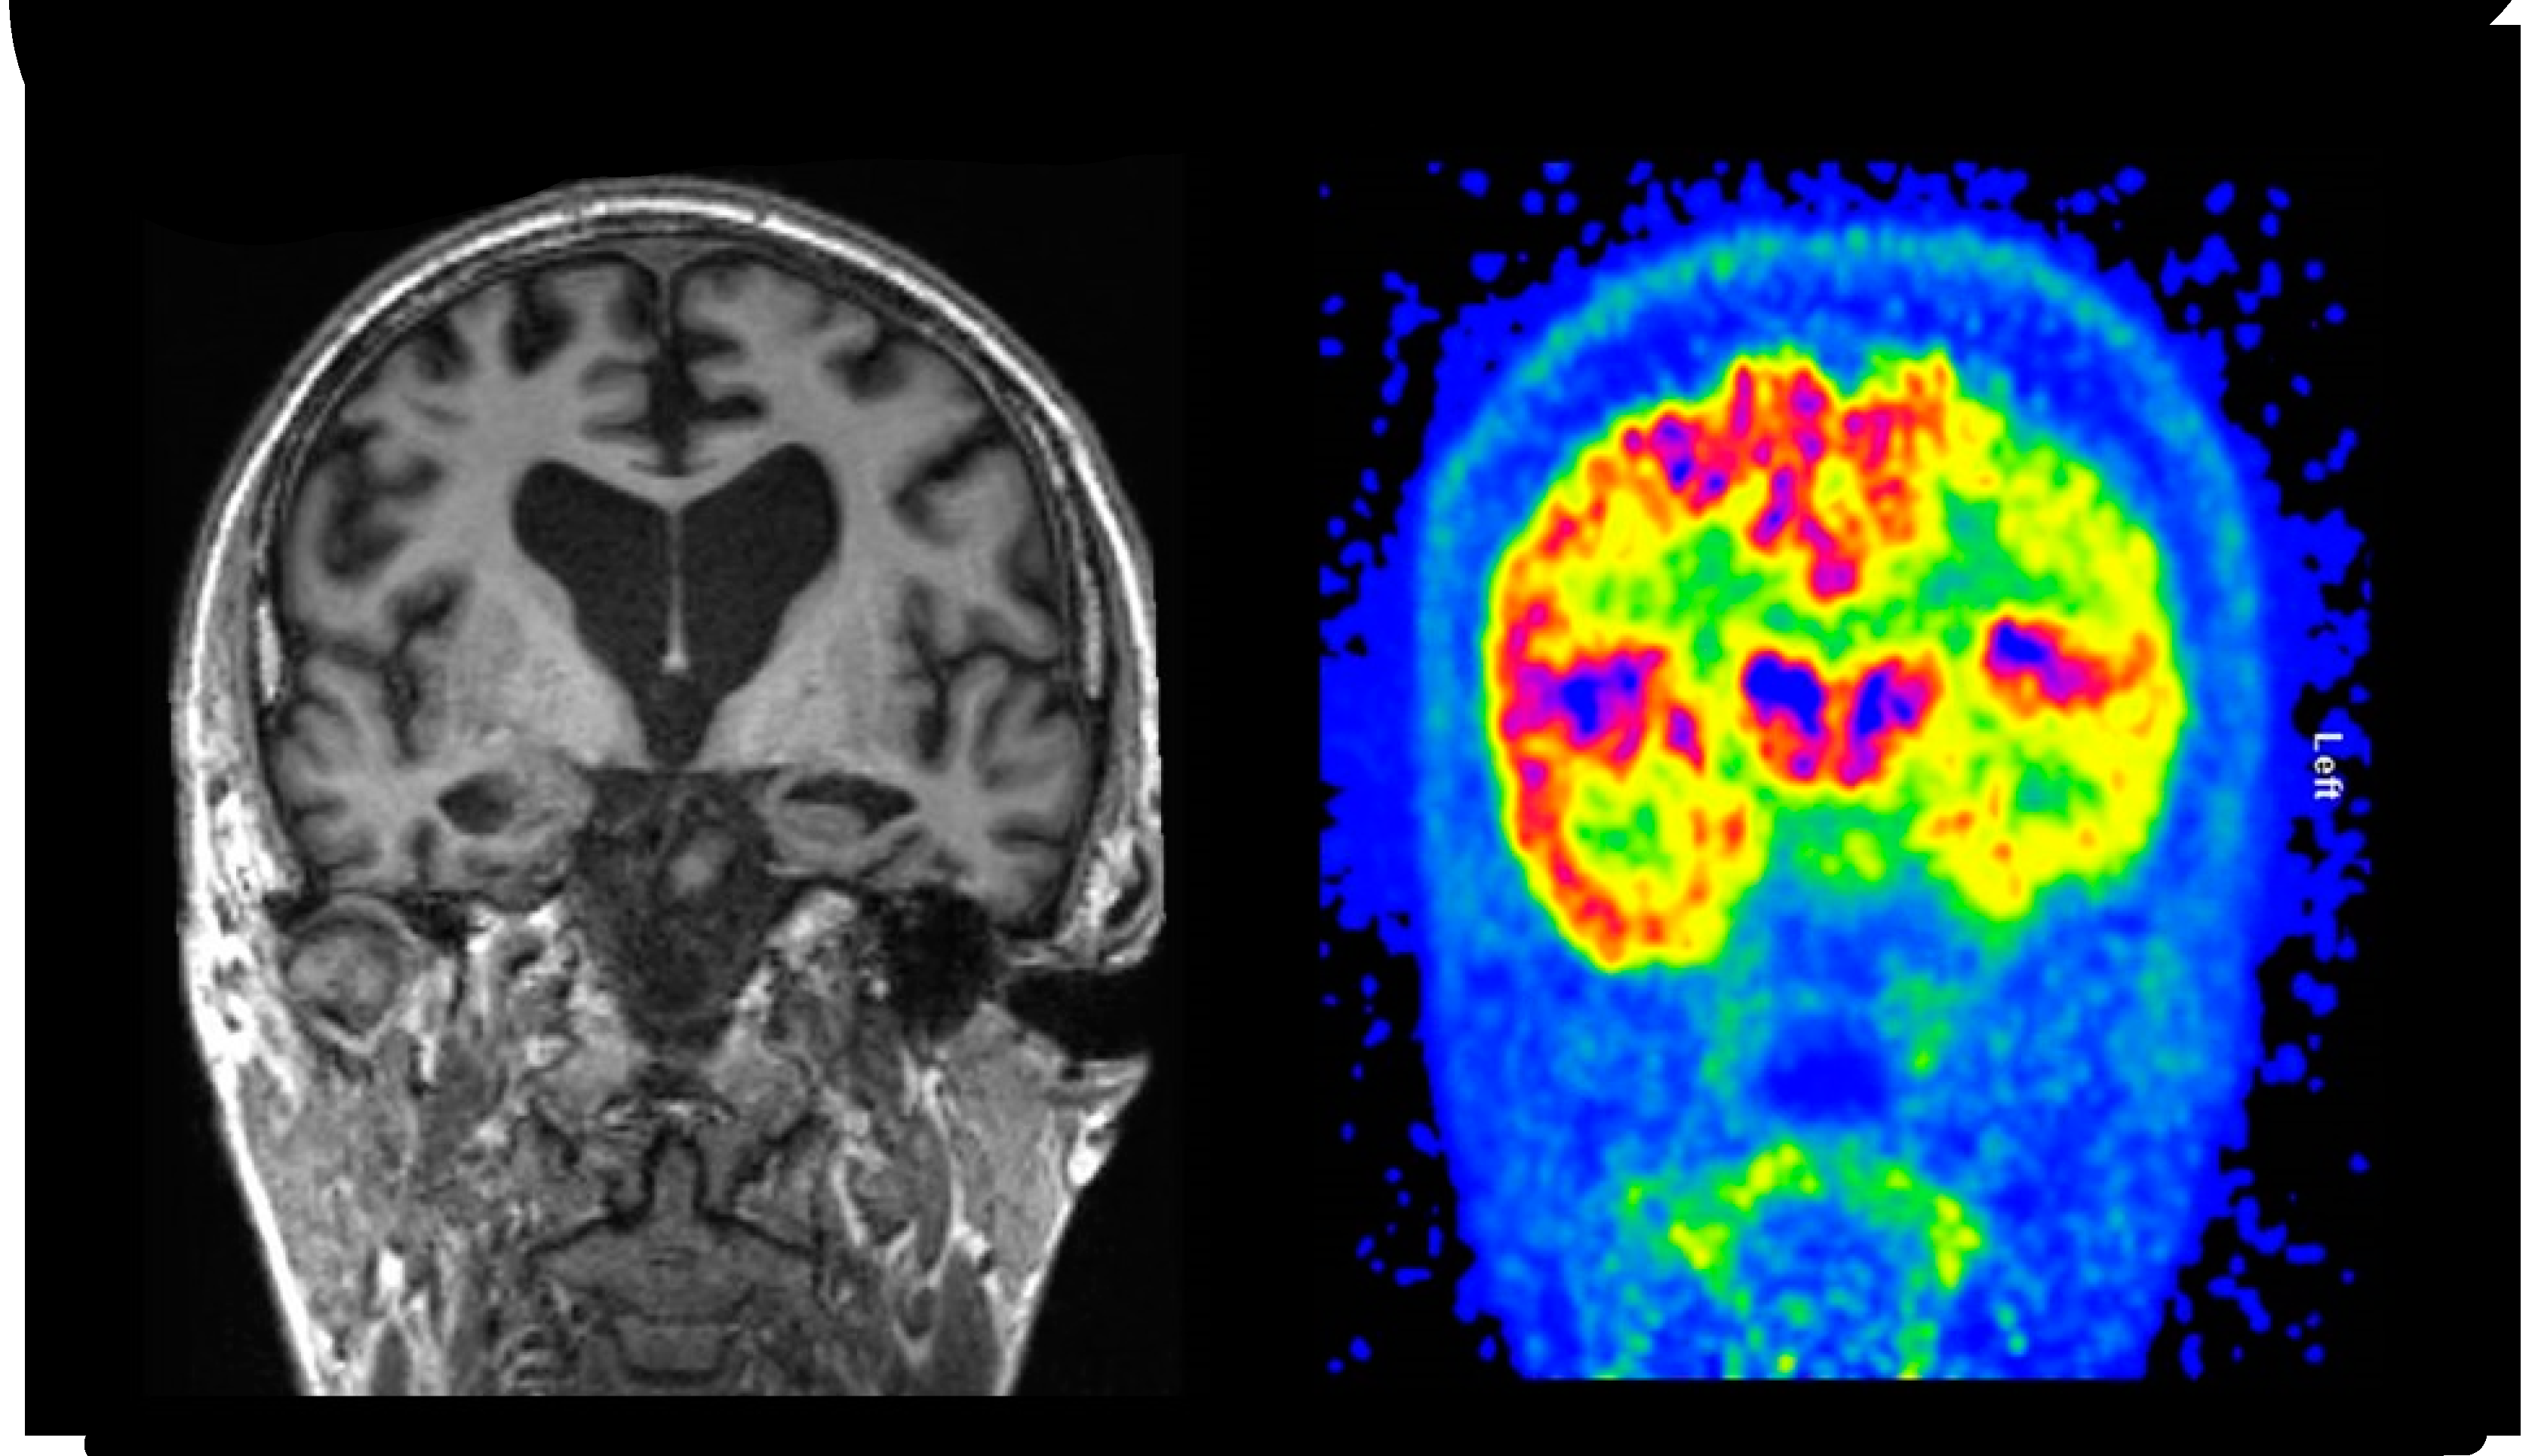
\includegraphics[
                    width=3.5cm,
                    trim={4cm 3cm 60cm 6cm},
                    clip
                ]{data/fdg_t1.png}
            };
            \node[label=below:{PET}] at (3, 0) {
                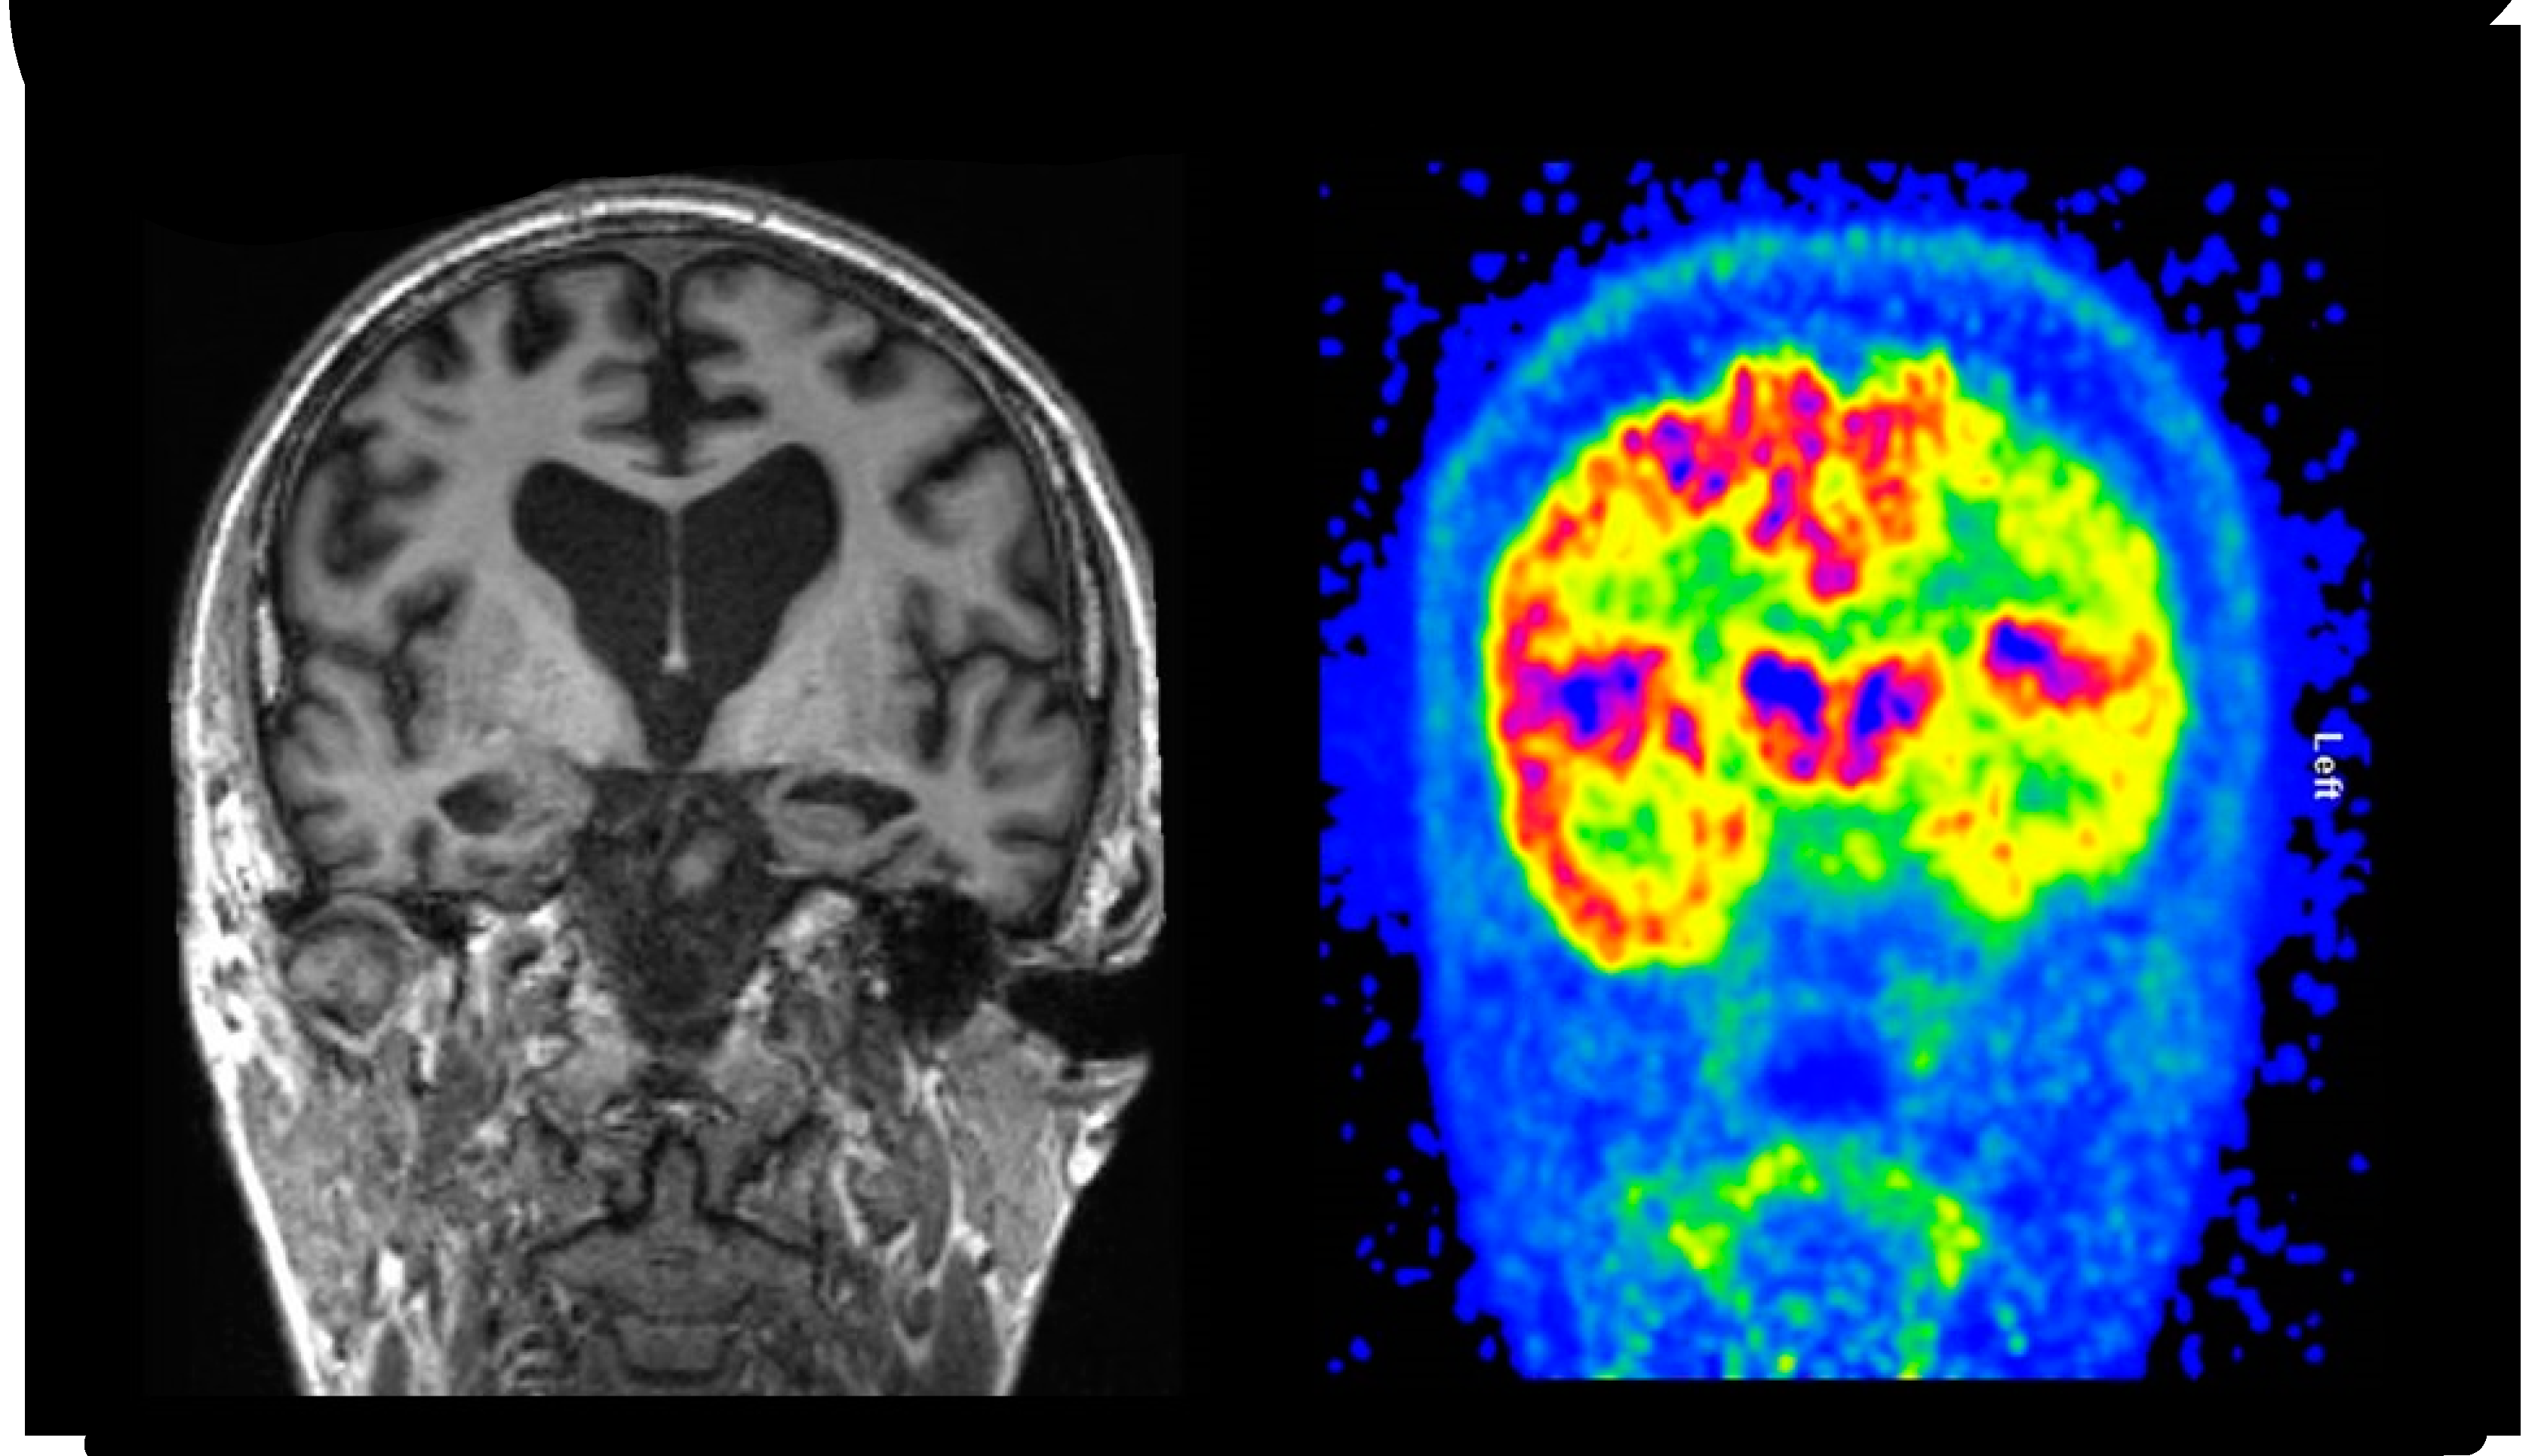
\includegraphics[
                    width=3.5cm,
                    trim={60cm 3cm 4cm 6cm},
                    clip
                ]{data/fdg_t1.png}
            };
        }
        \only<7>{
            \node[] at (-0.8, 0.5) {
                \dementia{2}
            };
        }
        \only<8>{
            \node[] at (-0.8, 0.5) {
                \dementia{3}
            };
        }
        \only<9>{
            \node[] at (-0.8, 0.5) {
                \dementia{4}
            };
        }
    \end{tikzpicture}
\end{frame}